\documentclass[letterpaper]{article}

\usepackage{natbib,alifeconf}
\usepackage{url,hyperref}
\usepackage{amsmath,amssymb}
\usepackage{booktabs}
\usepackage{array}

\newcommand\blfootnote[1]{%
  \begingroup
  \renewcommand\thefootnote{}\footnote{#1}%
  \addtocounter{footnote}{-1}%
  \endgroup
}

\newcommand{\full}{Ipsundrum+affect}
\newcommand{\readout}{Ipsundrum+affect (readout-only)}
\newcommand{\modulation}{Ipsundrum+affect (modulation-only)}
\newcommand{\Ns}{\ensuremath{N^s}}

\title{Where Does Affect Do the Work?\\
An ALife Decomposition of Evaluative Readout and Control Modulation in ReCoN-Ipsundrum}

\author{
    Aishik Sanyal$^{1}$ \\
    \mbox{}\\
    $^{1}$Xcellect, Canada \\
    aishik@xcellect.com
}

\begin{document}

\maketitle

\begin{abstract}
Minimal ALife agents are useful not because they settle consciousness attribution, but because they let us ask sharper questions about which architectural couplings generate indicator-like behavior. This paper extends the companion ReCoN-Ipsundrum architecture by decomposing its original ``affect coupling'' into two routes: direct evaluative readout into policy and affect-dependent modulation of recurrent control parameters. We compare three affect-enabled variants already supported in the public codebase: full coupling, readout-only, and modulation-only. The triplet is tested in three assays from the companion paper: familiarity-controlled corridor preference, reward-free exploratory play, and a pain-tail probe of post-stimulus planned caution. In the corridor, full coupling and readout-only retain high scenic choice even when the scenic branch is less novel (mean scenic-entry rate $0.94$ and $0.93$), while modulation-only is weaker ($0.86$). In exploratory play, modulation-only produces the widest roaming and highest scan count ($153.5$ viewpoints, $33.9$ scans), whereas readout-only produces the strongest local cycling (cycle score $10.15$ versus $0.10$ for modulation-only). In pain-tail, all three variants show long tails, but tail duration, salience-trace AUC, and turn-rate tail dissociate rather than collapsing onto a single marker. The result is a mechanism-decomposition study rather than a consciousness claim: evaluative readout and control modulation are not interchangeable, and architectural inspection matters for deciding which psychological descriptions a minimal simulation supports.
\end{abstract}

Submission type: \textbf{Full Paper}\\
Data/Code available at: \href{https://github.com/xcellect/recips}{github.com/xcellect/recips}
\blfootnote{\textcopyright~2026 Aishik Sanyal. Published under a Creative Commons Attribution 4.0 International (CC BY 4.0) license.}

\section{Introduction}
Minimal artificial agents are especially useful when the scientific target is not raw capability but the relation between \emph{architectural form} and the descriptions we attach to behavior. The companion ReCoN-Ipsundrum paper introduced an inspectable agent that extends a ReCoN state-machine substrate with a recurrent persistence loop over sensory salience and an optional affect proxy, and showed that adding affect coupling changes familiarity-controlled preference, exploratory play, and pain-tail behavior \citep{Sanyal2026ReCoNIpsundrum}. Yet ``affect coupling'' in that paper still bundled together two distinct possibilities: affective variables may enter behavior by being \emph{read out} directly into policy evaluation, or by \emph{modulating} the dynamics of the recurrent loop itself.

This extension separates those routes. The goal is not to make a stronger claim about machine consciousness. Instead, it asks a more ALife-like question: when a minimal agent exhibits marker-like behavior, \emph{where in the architecture does the relevant work happen}? That is a useful question even if the worlds are toy worlds and even if the answer remains local to this particular agent. It matters because behavior alone can be multiply realizable, while indicator-style interpretations are supposed to be linked to inspectable mechanisms rather than surface similarity alone \citep{ButlinEtAl2025Indicators}.

The extension produces a clean dissociation. In the corridor assay, stable scenic preference under novelty reversal tracks evaluative readout more than recurrent modulation. In exploratory play, modulation broadens roaming and scanning, while readout strengthens local cycling. In pain-tail, by contrast, no single behavioral metric cleanly belongs to just one route: tail duration, salience-trace persistence, and turning caution separate from one another. The philosophical payoff is modest but important: for minimal ALife models, the question is often not whether an agent ``has affect,'' but which coupling locus licenses which psychological description.

\section{Base Architecture and New Ablations}
ReCoN-Ipsundrum combines a Request Confirmation Network substrate \citep{BachHerger2015ReCoN} with a Humphrey-inspired recurrent ipsundrum loop over sensory salience and, when enabled, a simple Barrett-style affect proxy exposing valence, arousal, and body-budget error variables \citep{Humphrey2023Sentience,Barrett2017HowEmotions}. The full stage-wise construction, baseline comparisons against ReCoN and non-affective Ipsundrum, and the original multi-assay results are reported in the companion paper \citep{Sanyal2026ReCoNIpsundrum}. Here I keep the architecture fixed and only factor the affect-enabled model into two component-selective ablations.

\begin{table}[t]
\centering
\small
\begin{tabular}{@{}p{0.18\columnwidth}p{0.18\columnwidth}p{0.18\columnwidth}p{0.34\columnwidth}@{}}
\toprule
Variant & Readout into policy & Gain/precision modulation & Intended emphasis \\
\midrule
Full & on & on & both coupling routes \\
Readout-only & on & off & evaluation without control modulation \\
Modulation-only & off in base score & on & control modulation without direct evaluative weighting \\
\bottomrule
\end{tabular}
\caption{All three rows are affect-enabled Ipsundrum variants. ``Readout'' refers to direct use of valence, arousal, and body-budget error in the base action score.}
\label{tab:variants}
\end{table}

In code, the \readout{} variant leaves affect enabled but sets \texttt{modulate\_g=False} and \texttt{modulate\_precision=False}. The \modulation{} variant keeps affect-dependent gain and precision modulation active but zeros the main valence, arousal, and body-budget-error terms in the base score. This is a \emph{component-selective} decomposition rather than a mathematically pure severing: the policy also contains a small arousal-dependent forward-caution term and a curiosity-gating dependence on valence. The point, therefore, is to isolate the dominant route through which affective state shapes behavior, not to claim perfect causal purity.

\section{Assays and Experimental Setup}
I reuse three assays from the companion paper because they probe different candidate descriptions while keeping the worlds minimal and inspectable.

\textbf{Familiarity-controlled corridor preference.} The agent chooses between a scenic and a dull route that are equally safe. Pre-exposure manipulates which branch is familiar; the critical post condition is \emph{scenic familiar}, in which the scenic branch is less novel than the dull branch. I report scenic-entry rate and split-point novelty difference. Runs used $20$ seeds and $5$ post-familiarization mornings per seed.

\textbf{Reward-free exploratory play.} Agents roam for $200$ steps in a neutral-texture gridworld with curiosity enabled. I report unique viewpoints, scan events, cycle score, viewpoint entropy, and revisit rate. Runs used $20$ seeds and the built-in \texttt{ablation} config set.

\textbf{Pain-tail.} Each episode forces one hazard contact, removes the hazard, and then records planned actions for $200$ post-stimulus steps. I report tail duration, \Ns{} AUC above baseline, and mean turn-rate tail. Runs used $20$ seeds.

All numbers below are taken directly from the bundled \texttt{results/ablations} artifacts and the corresponding ALIFE engineering notes. Those notes also record the exact commands, the environment fixes required for plotting in a sandboxed setup, and a strict-mode test report of $36/36$ passing tests.

\begin{figure*}[t]
\centering
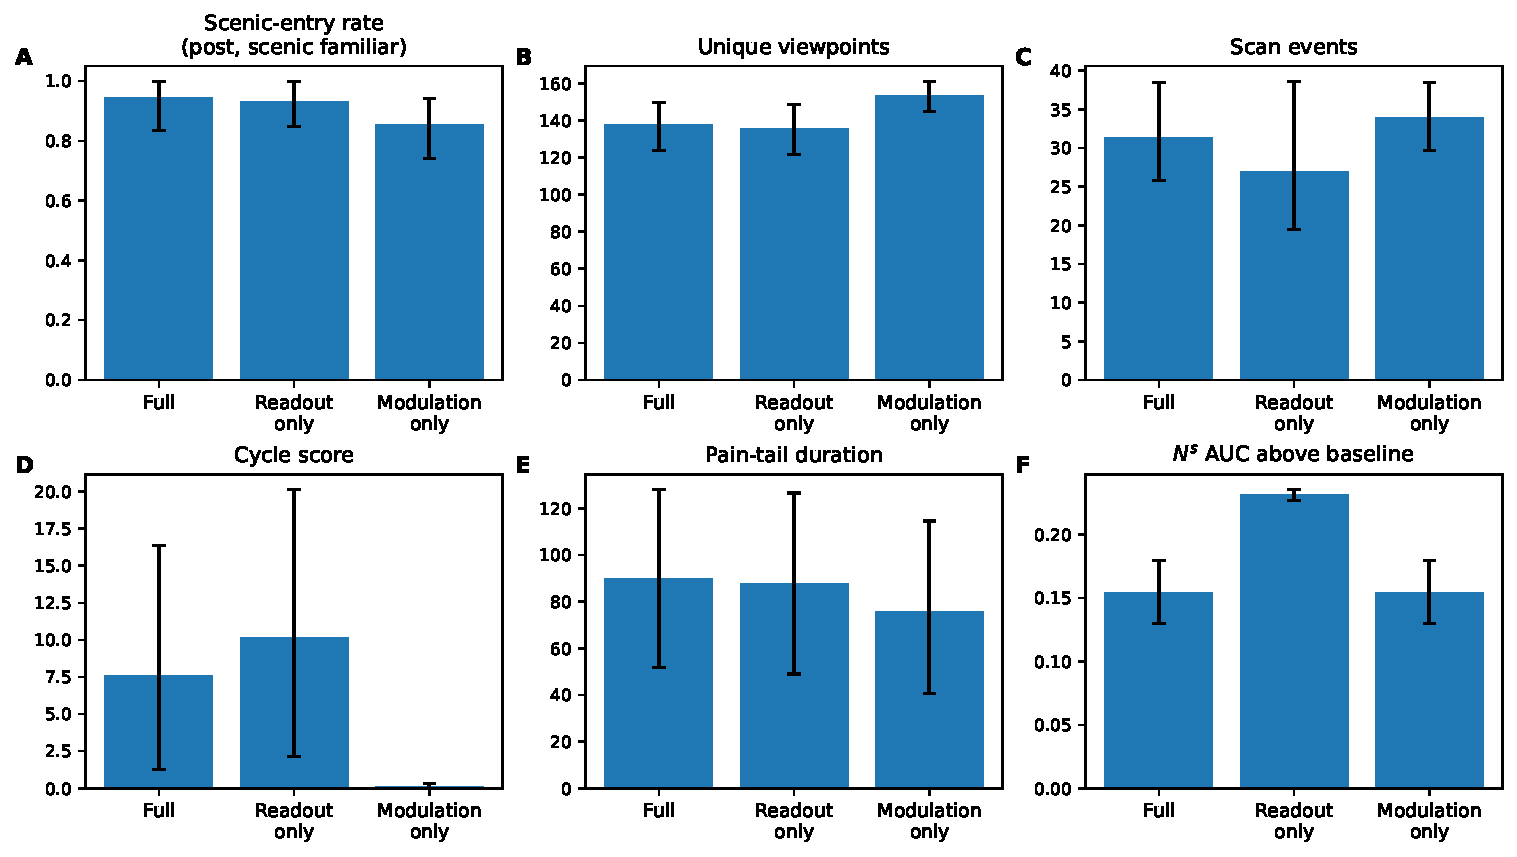
\includegraphics[width=0.99\textwidth]{alife_ablation_summary.pdf}
\caption{Ablation summary across the three assays. Error bars are $95\%$ bootstrap confidence intervals over per-seed means. Panels A--D show the main decomposition: stable scenic preference survives in full and readout-only variants, whereas exploratory breadth and scanning peak under modulation-only, and local cycling peaks under readout-only. Panels E--F show the more nuanced pain-tail result: long tails appear in all three variants, but tail duration and \Ns{} AUC above baseline do not pick out the same component.}
\label{fig:summary}
\end{figure*}

\section{Results}
\subsection{Stable preference tracks evaluative readout}
The corridor assay is the cleanest test of value-stable preference because the critical post condition makes the scenic branch \emph{less} novel than the dull branch. That reversal is visible in the split-point novelty metric for all three models: mean $\Delta$novelty is $-0.41$ for full coupling, $-0.40$ for readout-only, and $-0.35$ for modulation-only. Despite that disadvantage, scenic-entry rates remain high for \full{} ($0.94$ [$0.83$, $1.00$]) and \readout{} ($0.93$ [$0.85$, $1.00$]), but fall for \modulation{} ($0.86$ [$0.74$, $0.94$]).

The side-bias check points in the same direction rather than undermining it. Scenic choice stayed high on both left and right trials for all variants, with left/right scenic rates of $0.90/1.00$ for \full{}, $0.98/0.91$ for \readout{}, and $0.92/0.80$ for \modulation. The result is therefore not a trivial lane artifact. The most natural interpretation is that direct evaluative readout is doing most of the work in stabilizing scenic preference when novelty competes against it.

\subsection{Exploratory breadth tracks modulation, while local cycling tracks readout}
The exploratory-play assay yields the sharpest dissociation in the paper. \modulation{} produces the widest roaming profile: it achieves the highest unique-viewpoint count ($153.45$ [$145.15$, $161.40$]), the highest scan count ($33.90$ [$29.70$, $38.45$]), the highest viewpoint entropy ($7.09$ [$6.98$, $7.19$]), and the lowest revisit rate ($0.233$ [$0.193$, $0.274$]). By contrast, \readout{} produces the strongest local looping: its cycle score is $10.15$ [$2.15$, $20.15$], versus $7.60$ [$1.25$, $16.35$] for \full{} and essentially zero for \modulation{} ($0.10$ [$0.00$, $0.30$]).

This pattern matters because the older binary comparison---``with affect'' versus ``without affect''---could only tell us that affect coupling changes exploratory style. The new ablation triplet identifies \emph{how}. Modulation makes the agent range farther and scan more broadly; readout makes it more likely to settle into structured, revisiting local motifs. Full coupling sits between those poles, combining nonzero cycle structure with substantial breadth rather than maximizing either one alone.

\subsection{Pain-tail is the cautionary result, not the failure case}
Pain-tail is the place where a simple one-marker story breaks down. Tail duration alone does not isolate a single route: \full{} and \readout{} both show long mean tails ($89.85$ [$51.80$, $128.15$] and $87.80$ [$49.00$, $126.60$]), while \modulation{} is somewhat lower but still substantial ($75.95$ [$40.80$, $114.60$]). If we looked only at this measure, the decomposition would seem weak.

But the auxiliary metrics separate differently. \readout{} has the highest \Ns{} AUC above baseline ($0.232$ [$0.227$, $0.236$]), whereas \full{} and \modulation{} are both lower ($0.154$ [$0.130$, $0.179$]). Mean turn-rate tail shows a different ordering again: \full{} is highest ($0.703$ [$0.525$, $0.865$]), \modulation{} is similar ($0.690$ [$0.508$, $0.868$]), and \readout{} is lower ($0.608$ [$0.420$, $0.795$]). In other words, internal salience persistence and planned turning caution are not the same thing.

That is not an embarrassment for the decomposition. It is the most methodologically useful result in the extension. The earlier binary comparison invited the tempting gloss that lingering caution was a single signature of full affect coupling. The finer triplet shows that once we separate coupling loci, the pain-tail assay actually contains several partially independent phenomena.

\section{Discussion}
The extension supports three main lessons.

\textbf{First, evaluative readout and control modulation are not interchangeable.} The corridor and play assays both show that architecture matters at a finer grain than ``affect on'' versus ``affect off.'' Preference stability under novelty competition mostly follows readout, while exploratory breadth mostly follows modulation.

\textbf{Second, minimal ALife models are especially useful for \emph{locus} questions.} The point of these worlds is not that they are realistic enough to settle a consciousness attribution. The point is that they are simple enough to let us ask where a description is earned. In that sense, this paper is closer to an experimental philosophy of architectural description than to a consciousness demonstration.

\textbf{Third, single markers are unsafe.} Pain-tail shows why. Depending on whether one inspects tail duration, salience-trace persistence, or turning bias, the favored component changes. This is exactly the kind of underdetermination that motivates indicator programs to insist on multiple assays and architectural inspection rather than behavioral surface resemblance alone \citep{ButlinEtAl2025Indicators}.

The present decomposition still has clear limitations. The ablations are component-selective rather than fully pure, since small policy heuristics continue to reference affective variables outside the base score. The worlds are minimal and fixed-parameter, not developmental or open-ended. And the extension only compares affect-enabled variants; it sharpens the mechanism story of the companion paper rather than replacing the original baseline comparisons. The next step is therefore not a larger rhetorical claim, but a stronger robustness program: parameter sweeps, learned couplings, and tests of whether the same component dissociation survives outside these toy settings.

\section{Conclusion}
This paper refines the original ReCoN-Ipsundrum result by asking not whether affect coupling matters in general, but where it matters. The answer is not unitary. Readout matters most for stable evaluative preference and local cycling; modulation matters most for exploratory breadth and scanning; and pain-tail contains multiple partially independent effects rather than a single clean signature. For ALife, that is already a worthwhile outcome. It shows how minimal simulations can function as mechanism-decomposition tools: not proving consciousness, but clarifying which psychological descriptions are supported by which architectural couplings.

\bibliographystyle{apalike}
\bibliography{references}

\end{document}
